\documentclass[a4paper,12pt,portrait]{book}	  
\title{Mathematik f\"ur Physiker I}
\author{Friedemann Schuricht\\ \\ \"ubertragen von\\Lukas K\"orber und Friedrich Zahn}
\date{Wintersemester 2014/2015}

  
\usepackage[ngerman]{babel}	    
\usepackage[utf8]{inputenc}
\usepackage{amsmath}
\usepackage{mathtools}
\usepackage{amsthm}	 
\usepackage{graphicx}       % Einbinden von Bildern
\usepackage{lipsum,multicol}
\usepackage{fancyhdr}
\usepackage{xcolor}
\usepackage[upright]{fourier}
\usepackage[frak=mma]{mathalfa}
\usepackage{sectsty}
\usepackage{lipsum}
\usepackage{bm}
%\usepackage{MnSymbol} 

%define operators
\newcommand{\diff}[2]{\frac{\mathrm{d}{#1}}{\mathrm{d}{#2}}}
\newcommand{\ddiff}[2]{\frac{\mathrm{d}^2{#1}}{\mathrm{d}{#2}^2}}
\newcommand{\dddiff}[2]{\frac{\mathrm{d}^3{#1}}{\mathrm{d}{#2}^3}}
\newcommand{\ndiff}[2]{\frac{\mathrm{d}^n{#1}}{\mathrm{d}{#2}^n}}
\newcommand{\pdiff}[2]{\frac{\partial{#1}}{\partial{#2}}}

\newcommand{\Int}[4]{\int\limits_{#1}^{#2} #3 \mathrm{d} #4}
\newcommand{\Oint}[4]{\oint\limits_{#1}^{#2} #3 \mathrm{d} #4}

\newcommand{\bra}[1]{\left\langle #1 \right|}
\newcommand{\ket}[1]{\left| #1 \right\rangle}
\newcommand{\lara}[1]{\left\langle #1 \right\rangle}
\newcommand{\scap}[2]{\left\langle #1 \ \middle| \ #2\right\rangle}
\newcommand{\exlara}[3]{\left\langle #1 \ \middle| \ #2 \ \middle| \ #3\right\rangle}

\newcommand{\graph}{\text{graph\ }}
\newcommand{\rang}{\text{rang\ }}

\renewcommand{\sup}{\text{sup\ }}
\renewcommand{\inf}{\text{inf\ }}
\renewcommand\qedsymbol{$\textbf{q.e.d.}$}



\definecolor{dblue}{HTML}{183CE0}
\definecolor{hblue}{HTML}{0E75F7}
\sectionfont{\color{hblue}}
\chapterfont{\color{dblue}}

\newtheoremstyle{theoremstyle} % name
    {\topsep}                    % Space above
    {\topsep}                    % Space below
    {\upshape}                   % Body font
    {}                           % Indent amount
    {\sffamily\bfseries}                   % Theorem head font
    {}                          % Punctuation after theorem head
    {.5em}                       % Space after theorem head
    {\thmname{#1}\thmnumber{ #2}\thmnote{ (#3)}}  % Theorem head spec (can be left empty, meaning ‘normal’)

\theoremstyle{theoremstyle}
\newtheorem{theo}{Theorem}[section]
\newtheorem{sa}[theo]{Satz}
\newtheorem{lem}[theo]{Lemma}
\newtheorem{folgerung}[theo]{Folgerung}
\newtheorem*{definition}{Definition}
\newtheorem{beispiel}{Beispiel}

\newenvironment{theorem}
	{\par\nobreak\vfil\penalty0\vfilneg
   \vtop\bgroup\color{dblue}\noindent\rule{420pt}{2pt}\vspace{5pt}\begin{theo}}
	{\end{theo}\rule{50pt}{1pt}\color{black}\par\xdef\tpd{\the\prevdepth}\egroup
   \prevdepth=\tpd}
\newenvironment{satz}
	{\par\nobreak\vfil\penalty0\vfilneg
   \vtop\bgroup\color{dblue}\noindent\rule{420pt}{2pt}\vspace{5pt}\begin{sa}}
	{\end{sa}\rule{50pt}{1pt}\color{black}\par\xdef\tpd{\the\prevdepth}\egroup
   \prevdepth=\tpd}
\newenvironment{lemma}
	{\par\nobreak\vfil\penalty0\vfilneg
   \vtop\bgroup\color{dblue}\noindent\rule{420pt}{2pt}\vspace{5pt}\begin{lem}}
	{\end{lem}\rule{50pt}{1pt}\color{black}\par\xdef\tpd{\the\prevdepth}\egroup
   \prevdepth=\tpd}
	
\begin{document}
\maketitle
\tableofcontents
\pagestyle{fancy}
\renewcommand{\thechapter}{\Roman{chapter}} 
\renewcommand*\thesection{\arabic{section}}
\renewcommand\theequation{\maybe{\arabic{chapter}}\arabic{section}.\arabic{equation}}
\DeclareRobustCommand\maybe[1]{\ifnum#1=\value{chapter}\relax\else\uppercase\expandafter{\romannumeral#1}.\fi}
\setcounter{chapter}{7}


\chapter*{Überblick}
Diese Vorlesung wird sich mit folgenden Tehmen befassen:
    \begin{enumerate}
    \item \textbf{Integration auf Mannigfaltigkeiten}
    \item \textbf{Differenzialgleichungen}, sowohl gewöhnlich, als auch partiel
    \item \textbf{Funktionalanalysis} in Banach- und Hilberträumen (insbesondere
    unendlich dimensionale Räume z.B. von Folgen und Funktionen)
    \item \textbf{Funktionstheorie}, der Theorie von komplexwertigen Funktionen
    und z.B. $\mathbb{C}$-Differenzierbarkeit
    \end{enumerate}

\chapter{Integration auf Mannigfaltigkeiten}
\emph{Literaturtipp:} Königsberger Analysis 2, Springer
\setcounter{section}{28}

\section{Mannigfaltigkeiten}
Sei $\varphi\in C^q(V,\mathbb{R}^n)$ mit $q\in\mathbb{N}_{\geq 1}$, 
also $q$-fach stetig differenzierbar, wobei $V\subset\mathbb{R}^d$ offen ist, 
dann heißt $\varphi$ \textbf{regulär}, falls
    \begin{equation}
    \varphi'(x):\mathbb{R}^d\rightarrow\mathbb{R}^n \ \text{regulär (d.h. injektiv)}
    \end{equation}
Falls $\varphi$ regulär für alle $x\in V$ ist, heißt es auch 
\textbf{regulär auf V} beziehungsweise \\
\textbf{reguläre $C^q$-Parametrisierung} (manchmal auch $C^q$-Immersion). \\
$V$ ist dann der \textbf{Parameterbereich} von $\varphi$.\\
\emph{Bemerkung:} $\varphi(V)$ wird selten auch \textbf{Spur} von $\varphi$ genannt.\\
\linebreak
\linebreak
Aus der Linearen Algebra wissen wir, dass aus (29.1) sofort 
    \begin{equation}
    d\leq n
    \end{equation}
folgt. Dies sei in Kapitel VIII immer erfüllt! (29.2) ist außerdem äquivalent dazu, dass 
$\rang \varphi'(x)=d$.\\
    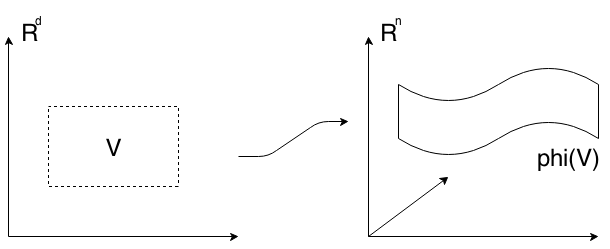
\includegraphics[scale=0.5]{pictures/MA2_0001}

\begin{beispiel}[reguläre Kurven $\varphi:I\subset\mathbb{R}\rightarrow\mathbb{R}^n$]
Dabei ist $I$ offen und der Tagentialvektor nirgendwo identisch mit dem Nullvektor, also 
$\varphi'(x)\neq 0$

\begin{enumerate}
    \item $\varphi:(0,2\pi)\rightarrow\mathbb{R}^2$ mit $\varphi(t)=\begin{pmatrix}
        \cos kt \\ \sin kt
    \end{pmatrix}$ und $k\in\mathbb{N}_{\geq 2}$\\

\begin{center}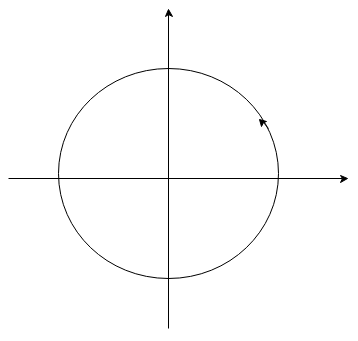
\includegraphics[scale=0.3]{pictures/MA2_0002}\\ 
\end{center}

Der Einheitskreis wird hier k-mal durchlaufen. 
Da $\varphi'(x)\neq 0$, ist $\varphi$ regulär.
\item $\varphi(-\pi,\pi)\rightarrow\mathbb{R}^2$ mit $\varphi(t)=(1+2\cos t)
    \begin{pmatrix}
    \cos t \\ \sin t
    \end{pmatrix}$\\

\begin{center}
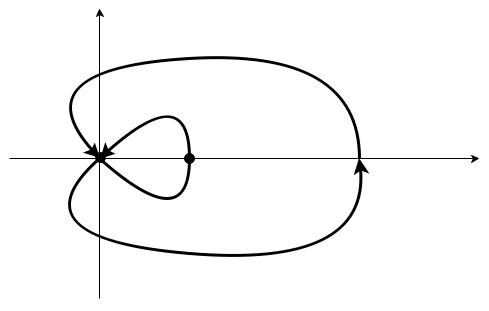
\includegraphics[scale=0.3]{pictures/MA2_0003}\\
\end{center}

$\varphi(\pm\frac{2\pi}{3})=
    \begin{pmatrix}
    0 \\ 0
    \end{pmatrix}
$, $ 
\varphi(0)=
    \begin{pmatrix}
    3 \\ 0
    \end{pmatrix}
$\\$
    \begin{pmatrix}
    1 \\ 0
    \end{pmatrix} $ 
\ gehört \textbf{nicht} zur Kurve ("$=\varphi(\pm\pi)$") und $\varphi$ ist regulär.

\item $\varphi:(-1,1)\rightarrow\mathbb{R}^2$ \ mit \ $\varphi(t)=\begin{pmatrix}
    t^3 \\ t^2
\end{pmatrix}$ \ ist wegen $\varphi'(0)=0$ \ \textbf{nicht} regulär\\

    \begin{center}
    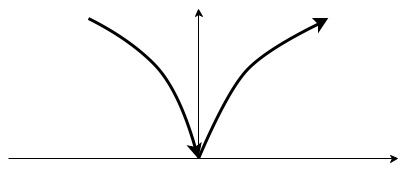
\includegraphics[scale=0.3]{pictures/MA2_0004}
    \end{center}

\end{enumerate}

\end{beispiel}
\ \linebreak

\begin{beispiel}[Parametrisierung von Graphen]
Sei $f\in C^q(V,\mathbb{R}^{n-d})$,\\
$V\subset\mathbb{R}^d$. Betrachtet wird $\varphi:V\rightarrow\mathbb{R}^n$ mit $\varphi(x)=(x,f(x))$\\
    \begin{center}
    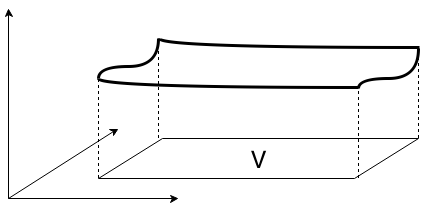
\includegraphics[scale=0.5]{pictures/MA2_0005}\\
    \end{center}
$\varphi$ ist regulär, da offenbar $\varphi\in C^q(V,\mathbb{R}^n)$ 
und $\varphi'=
    \begin{pmatrix} 
    id^d \\ 
    f'(x)
    \end{pmatrix}     
\in \mathbb{R}^{n \times d}$ \ ist.\\
\linebreak
\end{beispiel}

Es folgt eine Wiederholung zur \textbf{Relativtopologie} (vgl. Kapitel 14). Wir wissen, dass $U\subset M$ genau dann offen bezüglich $M$ ist, wenn es ein $\tilde{U}\subset\mathbb{R}^n$ gibt, dass offen ist, und das $U=\tilde{U}\cap M$ erfüllt. Später wird $M$ eine Mannigfaltigkeit sein und wir werden untersuchen, was in ihr offen ist.\\

\begin{center}
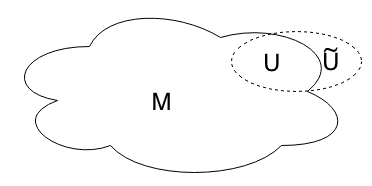
\includegraphics[scale=0.5]{pictures/MA2_0006}\\
\end{center}
Auf dieser Grundlage lässt sich auch der Begriff der \textbf{Umgebung} definieren:\\
$U\subset M$ heißt nämlich genau dann Umgebung von $u\in M$ bezüglich $M$, wenn es ein bezüglich $M$ offenes $U_0\subset M$ gibt, in dem $u$ liegt und das Teilmenge von $U$ ist.\linebreak\linebreak
\newpage
\textbf{\textsf{Beispiel für}} \ $M\subset\mathbb{R}^n$.\\

\begin{center}
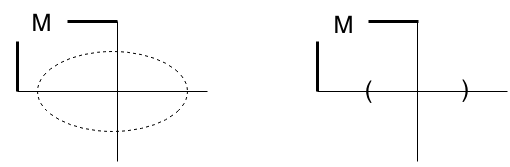
\includegraphics[scale=0.5]{pictures/MA2_0007}\\
\end{center}
\hspace{70pt} offen bzgl. M \hspace{70pt} nicht offen bzgl. M\\

\begin{definition}[Mannigfaltigkeiten]
Wir nennen $M\subset\mathbb{R}^n$ eine \textbf{d-dimensionale $C^q$-Mannigfaltigkeit} ($q\in\mathbb{N}_{\geq 1}$), falls

\begin{enumerate}
\item es für alle $u\in M$ eine (offene) Umgebung $U$ von $u$ bezüglich $M$ gibt und
\item es eine reguläre $C^q$-Parametrisierung $\varphi:V\subset\mathbb{R}^d\rightarrow\mathbb{R}^n$ ($V$ ist offen) existiert, die homöomorph ist und in die Mannigfaltigkeit abbildet (also \  $\varphi(V)=U$).
\end{enumerate}

\emph{Wiederholung: Eine stetige Abbildung heißt homöomorph, falls eine Umkehrabbildung existiert, die auch stetig ist.}\\
\end{definition}

In der Literatur wird $M$ auch manchmal als $C^q$-\emph{Unter}mannigfaltigkeit bezeichnet. Wir werden jedoch später zeigen, dass die verschiedenen Definitionen von Mannigfaltigkeiten gleichwertig sind.\\
Da ab jetzt immer hauptsächlich $C^1$-Mannigfaltigkeiten auftauchen werden, werden wir diese in Zukunft einfach "Mannigfaltigkeiten" nennen.\\

\begin{center}
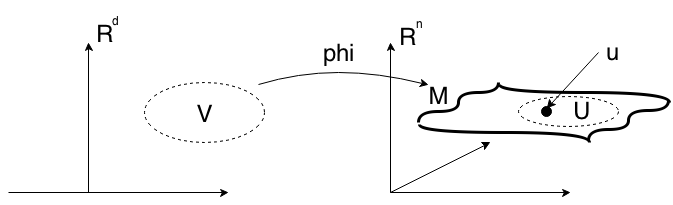
\includegraphics[scale=0.5]{pictures/MA2_0008}\\
\end{center}

Die Umkehrabbildung $\varphi^{-1}$ beziehungsweise ($\varphi^{-1}, U$) nennt man die \textbf{Karte} von $M$ um $u\in M$, wobei $U$ das zugehörige \textbf{Kartengebiet}, $\varphi$ selbst die Parametrisierung und $V$ der Parameterbereich ist.\\
Karten können eine Mannigfaltigkeit jedoch nur lokal beschreiben. Aus diesem Grund führt man den Begriff des Atlas, der eine globale Beschreibung ermöglicht, ein:\\
Die Menge $\{\varphi^{-1}_\alpha | \alpha\in A\}$ heißt \textbf{Atlas} der Mannigfaltigkeit M, falls die zugehörigen Kartengebiete $U_\alpha$ jene vollständig überdecken.\\
\linebreak
Weiterhin wichtig ist der Begriff der sogenannten \textbf{Einbettung}, bei der es sich um eine reguläre Parametrisierung handelt, die homöomorph ist. Wir vereinbaren, dass es sich im folgenden bei allen Parametrisierungen von Mannigfaltigkeiten stets um Einbettungen handelt.
\begin{beispiel}[Beweise bitte Selbstudium]\ \\

\begin{enumerate}
\item Der Kreis aus Beispiel 1.1 ist eine 1-dimensionale $C^\infty$-Mannigfaltigkeit, obwohl der Kreis k-fach durchlaufen wird. Der Atlas benötigt mindestens zwei Karten.
\item Die Kurven aus Biespiel 1.2 und 1.3 sind keine Mannigfaltigkeiten, da $\varphi$ nicht überall homöomorph ist.
\item Jedes offene $M\subset\mathbb{R}^n$ ist eine n-dimensionale $C^\infty$-Mannigfaltigkeit mit $\{id\}$ als Atlas.
\end{enumerate}
\end{beispiel}

\begin{beispiel} Sei $M:=\graph f$ aus Beispiel 2. Offenbar ist 
$\varphi:V\subset\mathbb{R}^d\rightarrow M\subset\mathbb{R}^n$ 
eine Einbettung. Das macht $M$ zu einer d-dimensionalen $C^q$-Mannigfaltigkeit.
\end{beispiel}

\begin{beispiel}
Sei $f:D\subset\mathbb{R}^n\rightarrow\mathbb{R}^{n-d}$ ($D$ offen) q-fach stetig differenzierbar für $q\geq 1$. Offenbar ist

\begin{equation}
\rang f'(u)=n-d \ \ \ \ \ \ \ \forall u\in D
\end{equation}
Wir nennen $M=\{u\in D \ | \ f(n)=0\}$ die Niveaumenge von $f$\\

\begin{center}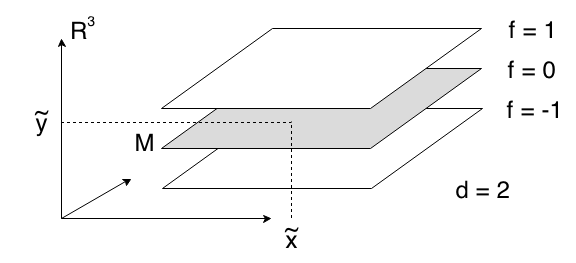
\includegraphics[scale=0.5]{pictures/MA2_0009}\\
\end{center}

Fixieren wir $\tilde{u}=(\tilde{x},\tilde{y})=(x_1,...,x_d,y_1,...,y_{n-d})\in M$
, so sehen wir mit (29.3) und eventuellen Koordinatenvertauschungen, dass 
$f(\tilde{x},\tilde{y})$ regulär ist. Der \emph{Satz über implizite Funktionen}
sichert uns nun, dass es eine Umgebung $V\subset\mathbb{R}^d$ von $\tilde{x}$, 
eine Umgebung $W\subset\mathbb{R}^{n-d}$ von $\tilde{y}$ und ein 
$\psi:V\rightarrow W\in C^q(V,W)$ gibt, das $(x,\psi(x))\in M$ erfüllt und homöomorph ist.\\
Es folgt, dass $\varphi:V\subset\mathbb{R}^d\rightarrow\mathbb{R}^n$ mit
$\varphi(x)=(x,\psi(x))$ eine homöomorphe, reguläre Einbettung  und $\varphi(V)$ 
Umgebung von $\tilde{u}\in M$ bezüglich von $M$ ist. Daraus können wir nun schließen, 
dass $M$ eine d-dimensionale $C^q$-Mannigfaltigkeit ist.\\
\linebreak
\emph{Bemerkung: $M=\graph f$ und $M=\{f=0\}$ sind grundlegende Konstruktionen 
für Mannigfaltigkeiten. \textbf{Lokal} ist jede Mannigfaltigkeit von dieser Gestalt!}
\end{beispiel}

\begin{sa}[lokale Darstellung einer Mannigfaltigkeit als Graph]
\mbox{} \\
Sei $M \subset \mathbb{R}^{n}$ eine d-dimensionale $C^{q}$-Mannigfaltigkeit. \\
$\Longleftrightarrow \forall u \in M \subset \mathbb{R}^n $ existiert eine Umgebung
$U$ von $u$  bezüglich $M$, $W \subset \mathbb{R}^n $ offen, 
$f \in C^q (W, \mathbb{R}^{n-d})$ und eine Permutation $\pi$ von Koordinaten in
$\mathbb{R}^n $ mit $ \psi (W) = U $ für $ \psi (v) \coloneqq \psi (v, f(v)) 
\forall v \in W $ (das heißt $U$ ist Graph von f).
\end{sa}

\textbf{somit:} $M$ ist $C^q$-Mannigfaltigkeit genau dann, wenn $M$ lokaler Graph
einer $C^q$-Funktion $f$ ist (vergleiche Beispiel 2 und 4).

\begin{proof}

$"\Leftarrow"$: folgt aus Beispielen 2 und 4. \\
$"\Rightarrow"$: fixiere $\tilde{u} \in M $, sei $\varphi : \tilde{V} \in \mathbb{R}^d
\rightarrow \tilde{U} \subset \mathbb{R}^n $ und der zugehörige $C^q$-Parameter 
$\tilde{u} = \varphi (\tilde{x})$ \\
$\varphi' (x)$ ist regulär $\xRightarrow{\text{ evtl. $\pi$ der Zeilen }} \varphi_I ' 
(\tilde{x}) \subseteq \mathbb{R}^{d \times d} $ ist regulär für $\varphi (x) =
    \begin{pmatrix}
    \varphi_I (x) \left[ \in \mathbb{R}^d \right]\\
    \varphi_{II} (x) \left[ \in \mathbb{R}^{n-d} \right]
    \end{pmatrix}
$ \\
Zerlege $u = \pi (v,w) $ mit $v \in \mathbb{R}^d $, 
d.h. $\tilde{u} = \pi (\tilde{v},\tilde{w})$

\textbf{Skizzen fehlen!}\\
$\xRightarrow{\text{Theorem über inverse Fkt.}} \exists V \subset \tilde{V} $ offen,
$\tilde{x} \in V, W \subset \mathbb{R}^d $ offen, $\tilde{v} \in W $
mit $\varphi_I ^{-1} : W \rightarrow V $ Homöomorphismus und $C^q$-Abbildung,
$\varphi_I ^{-1} (\tilde{v}) = \tilde{x} $ \\
mit $f(v) \coloneqq \varphi_{II} \left(\varphi_I ^{-1} (v)\right) \forall v \in W $ ist 
$f \in C^q \left(W, \mathbb{R}^{n-d}\right) $ \\
und $\psi (v) \coloneqq \varphi \left(\varphi_I ^{-1} (v) \right) =
\left( \varphi_I \left(\varphi_I ^{-1} (v) \right( ,
\varphi_{II} \left(\varphi_I ^ {-1} (v) \right) \right) = \pi \left(v, f(v)\right) $ \\
$\Rightarrow \psi (\tilde{v}) = \pi (\tilde{v}, \tilde{w}) = \tilde{u},
\psi (w) = \varphi (v) \in M \\
\varphi : \tilde{V} \rightarrow \tilde{U} $ ist Homöomorphismus \\
$\Rightarrow \varphi (v) $ ist offen in $M$ \\
$ \Rightarrow U \coloneqq \psi (W) $ ist offen bezüglich $M$
$\Rightarrow U $ ist Umgebung von $\tilde{u} $ bezüglich $M$ \\
$\xRightarrow{\tilde{u} \text{ beliebig}} $ Behauptung. 

\end{proof}

\begin{sa}[Charakterisierung von Mf mit umgebendem Raum]
\mbox{} \\
$M \subset \mathbb{R}^n $ sei d-dimensionale $C^q$-Mannigfaltigkeit. \\
$\Longleftrightarrow \forall u \in M $ existiert eine Umgebung $\tilde{U}$ von $u$ 
bezüglich $\mathbb{R}^n$, \\
$\tilde{V} \subset \mathbb{R}^n $, 
$\tilde{\psi}: \tilde{U} \rightarrow \tilde{V} $ wobei $\tilde{\psi} $ 
ein $C^q$-Diffeomorphismus ist und 
    \begin{equation*}
    \tilde{\psi} \left( \tilde{U} \cap M \right) =
    \tilde{V} \cap \left( \mathbb{R}^d \times {0} \right) 
    \end{equation*}

\textbf{Skizzen fehlen!}
\end{sa}

\textbf{Bemerkung:} Diese Charakterisierung von Mannigfaltigkeiten benutzt den umgebenden Raum und wird häufig als Definition der Mannigfaltigkeit benutzt.    
    
\begin{proof}
$"\Leftarrow"$: $\psi $ eingeschränkt auf $\tilde{U} \cap M $ liefert Karten 
$\Rightarrow$ Behauptung. \\
$"\Rightarrow"$: fixiere $\tilde{u} \in M $, wähle $\tilde{U} \subset M $,
$W \subset \mathbb{R}^d $, $f \in C^q \left( W, \mathbb{R}^{n-d} \right)$ \\
gemäß Satz 29.1 oBdA $\pi = $ \textit{id} \\
zerlege $u = (v,w) \in \mathbb{R}^d \times \mathbb{R}^{n-d}$, 
$\tilde{u} = \left( \tilde{v}, f \left( \tilde{v} \right) \right) $ \\
sei $\hat{U} \coloneqq W \times \mathbb{R}^{n-d} \eqqcolon \hat{V} $,
liefert "Zylinder" aus $U$ und $W$ in Beweis zu Satz 29.1 \\
sei $\tilde{\varphi}: \hat{V} \rightarrow \hat{U} $ mit
$\tilde{\varphi} (v,w) \coloneqq (v, f(v) + w) \Rightarrow \tilde{\varphi} \in C^q $ \\
$\tilde{\varphi}' \left( \tilde{v}, 0 \right) =
    \begin{pmatrix}
    \textit{id}_d & 0 \\
    f'(v)         & \textit{id}_{n-d}
    \end{pmatrix}
$ ist regulär \\
$\xRightarrow{\text{Satz ü. inverse Fkt.}} \exists $ 
Umgebung $ \tilde{U} \subset \hat{U}$ von $\tilde{U}$,
Umgebung $ \tilde{V} \subset \hat{V} $ von $ \left( \tilde{v}, 0 \right) $, sodass \\
$\tilde{\psi} \coloneqq \tilde{\varphi}^{-1} \in C^q \left( \tilde{U}, \tilde{V} \right) $
exisitiert. \\
wegen $\tilde{\varphi} \left( \tilde{V} \cap \left( \mathbb{R}^d \times {0} \right) \right)
= \tilde{U} \cap M $ folgt die Behauptung.
\end{proof}

\begin{folgerung}
Sei $M \subset \mathbb{R}^n$ d-dimensionale $C^q$-Mannigfaltigkeit \\
und $\varphi: V \subset \mathbb{R}^d \rightarrow U \subset M $ Parameter um $u \in M $ \\
$\Longrightarrow \exists \tilde{U}, \tilde{V} \subset \mathbb{R}^n $ offen und 
$\tilde{\varphi} : \tilde{V} \rightarrow \tilde{U} $ 
mit $ U \subset \tilde{U}, V \times {0} \subset \tilde{V} $, \\
$\tilde{\varphi} $ ist $C^q$-Diffeomorphismus und
$\tilde{\varphi} (x, 0) = \varphi (x) \forall x \in V $
\end{folgerung}

\begin{proof}
Folgt aus Beweisen von Satz 29.1 und 29.2
\end{proof}

\begin{theo}[lokale Darstellung von Mf als Niveaumenge]
\mbox{} \\
$M \subset \mathbb{R}^n $ sei d-dimensionale $C^q$-Mannigfaltigkeit. \\
$\Longleftrightarrow \forall u \in M $ existiert eine Umgebing $\tilde{U}$ von $u$
bezüglich $\mathbb{R}^n$ und \\
$f \in C^q \left( \tilde{U}, \mathbb{R}^{n-d} \right)$ 
mit $\textit{rang } f' (u) = n-d $ und \\
$\tilde{U} \cap M = \left\lbrace \tilde{u} \in \tilde{U} | f (\tilde{u}) = 0 \right\rbrace $
\end{theo}

\textbf{somit:} $M$ ist eine $C^q$-Mannigfaltigkeit genau dann, 
wenn $M$ die lokale Niveaumenge einer $C^q$-Funktion $f$ ist. \\

\textbf{Bemerkung:} $c \in \mathbb{R}^{n-d} $ heißt \textit{regulärer Wert} von
$f \in C^q \left( \tilde{U}, \mathbb{R}^{n-d} \right) $, \\
$\tilde{U} \subset \mathbb{R}^n $
offen, falls $\textit{rang } f' (u) = n-d \forall u \in \tilde{U} $ mit $f(u) = c $ \\
Folglich ist $M \coloneqq \left\lbrace u \in \tilde{U} | f(u) = c \right\rbrace $ 
eine d-dimensionale $C^q$-Mannigfaltigkeit, falls $c$ ein regulärer Wert von $f$ ist.

\begin{proof}
$"\Leftarrow":$ gemäß Bsp. 5 erhält man lokale Parametriesierung \\
$\Rightarrow$ Behauptung. \\
$"\Rightarrow":$ fixiere $\tilde{u} \in M$, 
wähle $\tilde{U}, \tilde{V} \subset \mathbb{R}^n, 
\tilde{\psi}: \tilde{U} \rightarrow \tilde{V} $ gemäß Satz 29.2 \\
sei $f \coloneqq \left( \tilde{\psi}_{d+1}, \ldots , \tilde{\psi}_n \right)$,
offenbar $f \in C^q \left(  \tilde{U}, \mathbb{R}^{n-d} \right) $ \\
mit $\tilde{\psi}$ aus dem Beweis zu Satz 29.2:
$\tilde{\psi}' (\tilde{u}) = \tilde{\varphi}' (\tilde{v}, 0)^{-1} $ ist regulär \\
$\Rightarrow f'(\tilde{u}) $ hat vollen Rang, d.h. $\textit{rang } f'(\tilde{u}) = n-d $ \\
nach Konstruktion $ \left\lbrace u \in \tilde{U} | f(u) = 0 \right\rbrace = U \cap M
\Rightarrow $ Behauptung.
\end{proof}

\begin{lem}[Kartenwechsel] 
\mbox{} \\
Sei $M \in \mathbb{R}^n $ d-dimensionale Mannigfaltigkeit \\
und $\varphi_1^{-1}, \varphi_2^{-1} $ Karten mit zugehörigem Kartengebiet 
$U_1 \cap U_2 \neq \emptyset $ \\
$\Longrightarrow 
\varphi_2^{-1} \circ \varphi_1 : \varphi_1^{-1} \left( U_1 \cap U_2 \right)
\rightarrow \varphi_2^{-1} \left( U_1 \cap U_2 \right) $ ist $C^q$-Diffeomorphismus.

\textbf{Skizze fehlt!}
\end{lem}

\begin{proof}
Ersetze $\varphi_1, \varphi_2 $ mit $\tilde{\varphi}_1, \tilde{\varphi}_2 $
gemäß Folgerung 29.3 \\
$\Rightarrow$ Einschränkung von $\tilde{\varphi}_2^{-1} \circ \tilde{\varphi}_1 $
liefert Behauptung. 
\end{proof}

\begin{definition}
Sei $M \subset \mathbb{R}^n $ d-dimensionale Mannigfaltigkeit. \\
Ein Vektor $v \in \mathbb{R}^n $ heißt \textbf{Tangentialvektor} in $u \in M $ an $M$, \\
falls eine stetig differenzierbare Kurve 
$\gamma: (-\delta, \delta) \rightarrow M (\delta > 0) $ exisitiert mit \\
$\gamma (0) = u $ und $\gamma' (0) = v $. \\
Die Menge aller Tangentialvektoren $T_uM$ heißt Tangentialraum.
\end{definition}

\begin{sa}
Sei $M \in \mathbb{R}^n $ eine d-dimensionale Mannigfaltigkeit, \\
$u \in M $, $ \varphi : V \rightarrow U $ der zugehörige Parameter um $u$ \\
$\Longrightarrow T_uM $ ist d-dimensionaler $( \mathbb{R}-) $ Vektorraum und \\
    \begin{equation}
    T_uM = \underbrace{\varphi'(x)}_{L \left( \mathbb{R}^d, \mathbb{R}^n \right) }
    \left( \mathbb{R}^d \right) \text{ für } x = \varphi^{-1} (u) 
    \end{equation}
wobei $T_uM$ unabhängig vom speziellen Parameter $\varphi$ ist.
\end{sa}

\begin{proof}
Sei $\gamma: (-\delta, \delta) \rightarrow M eine C^1$-Kurve mit $\gamma(0) = u $ \\
$\Rightarrow g \coloneqq \varphi^{-1} \circ \gamma $ ist $C^1$-Kurve, 
$g: (-\delta, \delta) \rightarrow \mathbb{R}^d $ mit $ g(0) = x $ und
    \begin{equation*}
    \gamma' (0) = \varphi' (x) g'(0) \text{, } \varphi' (x) \text{ist regulär.}
    \tag{$\spadesuit$}
    \end{equation*}
Offenb. liefert auch jede $C^1$-Kurve $g$ in $\mathbb{R}^d $ durch $x$
eine $C^1$-Kurve $\gamma$ in $M$ mit $(\spadesuit)$ \\
Die Menge aller Tangentialvektoren $g'(0)$ von $C^1$-Kurven $g$ in $\mathbb{R}^d $
ist offenbar $\mathbb{R}^d $ \\
$\Rightarrow $ 
29.4 $ \xRightarrow{\varphi' (x) \text{ ist regulär}} \textit{dim } T_uM = d $ \\
da $(\spadesuit)$ für jeden Parameter $\varphi$ gilt, ist $T_uM$ unabhängig von $\varphi$.
\end{proof}

\textbf{Bemerkung:}
\par \noindent
Man bezeichnet auch $(u, T_uM) \subset M \times \mathbb{R}^n$
als Tangentialraum und \\
$TM = \bigcup\limits_{U \in M} (u, T_uM) \subset M \times \mathbb{R}^n $
als Tangentialbündel.

\begin{beispiel}
Sei $M \subset \mathbb{R}^n $ offen  \\
$\Rightarrow $ $M$ ist ist n-dimensionale Mannigfaltigkeit und 
$T_uM = \mathbb{R}^n \forall u \in M $
\end{beispiel}

\begin{definition}
Sei $M \subset \mathbb{R}^n $ d-dimensinale Mannigfaltigkeit. \\
Ein Vektor $w \in \mathbb{R}^n $ heißt \textbf{Normalenvektor} in $u \in M $ an $M$, falls\\
$\langle w,v \rangle = 0 \forall v \in T_uM $
(d.h. $w \bot v \forall v \in T_uM$) \\
Die Menge aller Normalenvektoren $N_uM = T_uM^{\bot} $ heißt \\
\textbf{Normalenraum} von $M$ in $u$. 
\end{definition}

\end{document}